\documentclass[a4paper,12pt]{article}
\usepackage{ctex} %支持中文
\usepackage{geometry} %页面
\usepackage{amsmath} %公式
\usepackage{graphicx} % 图片
\usepackage{color} %字体等颜色

\title{质量、动量与能量守恒方程公式推导}
\author{孙俊博}
% 页边距
\geometry{a4paper,left=2.5cm,right=2.5cm,top=2.5cm,bottom=2.5cm}
% 行距
\linespread{1.5}
\begin{document}
\maketitle{}

\begin{abstract}
详细地阐述质量、动量与能量守恒方程的推导过程,以便后续查看与记忆。文章的具体内容包括:\par
质量守恒方程的推导,其中包括对于微元体各个面的质量流量的推导,以及最终公式的推导与化简;\par
动量守恒方程的推导,以最基本的牛顿第二定律为理论基础,推导流体微元所受到的质量力(或称体积力)与表面力,以及流体微元的加速度——速度的随体导数,得出的应力形式的动量守恒方程,随后,将应力形式动量守恒方程中的应力变量(包括正应力与切应力)转换为公式中其它已有的变量(以消除部分未知量),最后给出动量守恒方程的最终形式;\par
\textbf{这里还需要补充能量守恒方程的简要摘要}
\end{abstract}

\section{基础知识}
	此部分的主要内容,是为后续三个公式的推导打下基础,简要阐述一些数学或物理上的定理、公式等,包括泰勒展开式、随体导数等。以及一些基本常识。另外也阐述了三个方程推导所通用的方法。\par

	\subsection{泰勒展开式}
		泰勒展开式的中心思想,个人通俗的理解为:使用一个万能公式,去近似的表示(或替代)另一个公式,用一个已知的信息的状态,去近似的逼近另一个未知的状态,这在后续斗有所体现,其数学上单一变量的公式为:\par
		\begin{equation}
			f(x)=\sum_{n=0}^{\infty} \frac{f^{(n)}(x)}{n!} {(x-x_{0})}^{n}
		\end{equation}

	\subsection{随体导数}
		随体导数的概念理解可以借助一些形象的例子,如人的心情emotion,是受到很多因素的影响的,它会受到时间的影响,也会受到某些事件的影响,但总体上可以概括为受到时间与地点两种基本因素的影响,如在南京的心情会好一些,在纽约的心情则会差一些,而早上的心情会好一些,到了傍晚人们有时会有些低落。\par
		流体中的许多变量,也有这种特性,最为常见的就是流体质点的流速,一条河流的上游与下游流速不同,由于潮汐作用,早上与晚上即便是同一地点的流速或者流向也不相同,这种现象可以用公式概括为:\par
		\[
			\vec{u}=f(x,y,z,t)
		\] \par
		在三维空间中,对于加速度a就是 $\vec{u}$ 的全导数,其公式为:
		\[
			\frac{D \vec{u}}{Dt} = \frac{\partial \vec{u}}{\partial t}
		+\frac{\partial \vec{u}}{\partial x} \cdot \frac{\partial x}{\partial t}
		+\frac{\partial \vec{u}}{\partial y} \cdot \frac{\partial y}{\partial t}
		+\frac{\partial \vec{u}}{\partial z} \cdot \frac{\partial x}{\partial t}
		\] \par
		而各个方向上,位移对时间的导数如$\frac{\partial x}{\partial t}$即是x方向上的速度u,因此上式可简化为:
		\begin{equation}
			\frac{D \vec{u}}{Dt} = \frac{\partial \vec{u}}{\partial t}
			 =\frac{\partial \vec{u}}{\partial t}
			 +u\frac{\partial \vec{u}}{\partial x}
			 +v\frac{\partial \vec{u}}{\partial y}
			 +w\frac{\partial \vec{u}}{\partial z}
		\end{equation} \par

	\subsection{方程推导通用方法}
对于质量、动量、能量守恒方程,三者都用到了截面通量的推导方法,详细内容可根据下图进行叙述:\par
\begin{figure}[htbp]
	\centering
	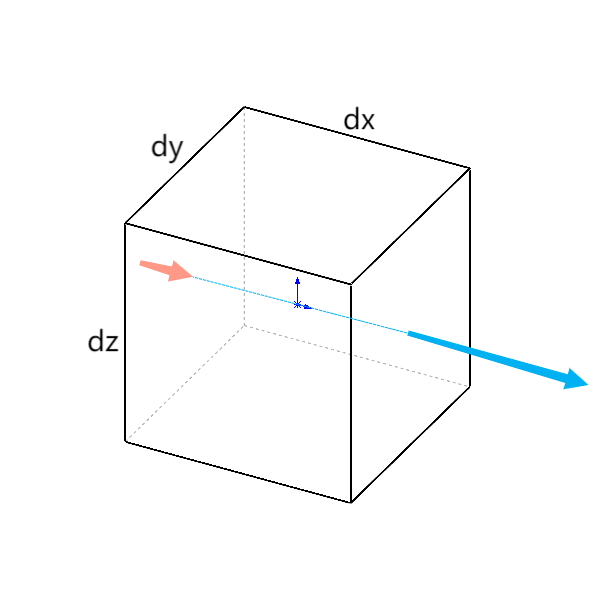
\includegraphics[width=0.5\textwidth,height=0.5\textwidth]{cube.png}
	\caption{流体微元物理量通量示意图}
	\label{流体微元示意}
\end{figure}\par
假设一物理量(如速度)按照流体微元\textcolor{red}{红色}从左侧垂直流入微元,量记为u,那么在x方向上,只要流体微元足够小,那么流体微元这一物理量在x方向上的变化就可以视作线性的,则在\textcolor{blue}{蓝色}出口面上,这一物理量的数值将会变为多少呢?将会变为该物理量进口面的数值+(斜率乘以两个面的距离),为$u+\frac{\partial u}{\partial x} \cdot dx$,而泰勒展开可以得到相同的答案,但个人认为这种理解更加简单易于理解。那么在x方向上,这一物理量的通量$\Phi$为\textcolor{red}{红色}物理量通量减去\textcolor{blue}{蓝色}物理量通量,即:
		\begin{equation}
		\varPhi=u\cdot dx\cdot dydz-(u+\frac{\partial u}{\partial x} )\cdot dx \cdot dydz-=-\frac{\partial u}{\partial x} \cdot dxdydz
		\end{equation} \par
		这一结果将会在续后每个公式的推导过程中使用到,届时只需要将u换成后续推导过程中的物理量即可。需要说明的是,上述方程中使用偏导$\partial$的原因是因为流入该截面的物理量不一定垂直于该截面,而方程只阐述了垂直于该截面的物理量分量而已。
\section{质量守恒方程}
	质量守恒的核心思想是:一个控制体的质量M不会无缘无故地增加或者减少,其变化是因为质量的流入量与流出量产生了差异,用公式可以表示为:
	\[
	\Delta M=Q_{m\_in}-Q_{m\_out}
	\] \par
	\textbf{在等式左边}:对于$\Delta M$有\[\Delta M=\frac{dM}{dt}=\frac{d\rho}{dt} \cdot dxdydz\] \par
	\textbf{在等式右边}:对于$Q_{m\_in}-Q_{m\_out}$,可以使用$m=\rho V$ 进行计算,其中的$\rho V$可以理解为物理量密度与速度的乘积在一个截面上的通量,则在x方向上,根据公式(3)即有:
	\[
	(Q_{m\_in}-Q_{m\_out})_{x}=-\frac{\partial (\rho u_{x})}{\partial x} \cdot dxdydz
	\] \par
	同理在y方向与z方向则有
	\[
	(Q_{m\_in}-Q_{m\_out})_{y}=-\frac{\partial (\rho u_{y})}{\partial y} \cdot dxdydz
	\]

	\[
	(Q_{m\_in}-Q_{m\_out})_{z}=-\frac{\partial (\rho u_{z})}{\partial z} \cdot dxdydz
	\] \par
	汇总则有:
	\[
	\begin{aligned}
	(Q_{m\_in}-Q_{m\_out}) & =(Q_{m\_in}-Q_{m\_out})_{x}+(Q_{m\_in}-Q_{m\_out})_{y}+(Q_{m\_in}-Q_{m\_out})_{z} \\ &
	=-\frac{\partial (\rho u_{x})}{\partial x} \cdot dxdydz-\frac{\partial (\rho u_{y})}{\partial y} \cdot dxdydz-\frac{\partial (\rho u_{z})}{\partial z} \cdot dxdydz \\ &
	=-[\frac{\partial (\rho u_{x})}{\partial x}+\frac{\partial (\rho u_{y})}{\partial y}+\frac{\partial (\rho u_{z})}{\partial z}]dxdydz
	\end{aligned}
	\]

	左边=右边,则有:
	\[
		\frac{d\rho}{dt} \cdot dxdydz +[\frac{\partial (\rho u_{x})}{\partial x}+\frac{\partial (\rho u_{y})}{\partial y}+\frac{\partial (\rho u_{z})}{\partial z}]dxdydz=0
	\] \par
	化简有:
	\begin{equation}
			\frac{d\rho}{dt} + \frac{\partial (\rho u_{x})}{\partial x}+\frac{\partial (\rho u_{y})}{\partial y}+\frac{\partial (\rho u_{z})}{\partial z}=0
	\end{equation} \par
	向量形式为:
	\[
\frac{d\rho}{dt} +\nabla \cdot (\rho \vec{V})=0
\] \par

\section{动量守恒方程}

\section{能量守恒方程}
\end{document}